\documentclass[11pt,a4paper]{article}
\usepackage[margin=1in]{geometry}
\usepackage{graphicx}
\usepackage{hyperref}
\usepackage{listings}
\usepackage{xcolor}
\usepackage{caption}
\usepackage{booktabs}
\usepackage[section]{placeins}

\lstset{
  basicstyle=\ttfamily\small,
  breaklines=true,
  frame=single,
  backgroundcolor=\color{gray!8}
}

\title{LSV 2026 Programming Assignment 1\\Report}
\author{Wei-Hung Chan, R15921041}
\date{\today}

\begin{document}
\maketitle

\section{Exercise 2: Using ABC}

\subsection{2(a) Two-bit unsigned multiplier BLIF}

The file \texttt{lsv/pa1/mul.blif} implements $Y = A \times B$ where
$A=(a_1 a_0)$, $B=(b_1 b_0)$, and $Y=(y_3 y_2 y_1 y_0)$.
Partial products are formed first, then the product bits:

\begin{lstlisting}
p00 = a0 & b0;   p01 = a0 & b1;
p10 = a1 & b0;   p11 = a1 & b1;
y0 = p00;
y1 = p01 XOR p10;   c1 = p01 AND p10;
y2 = p11 XOR c1;    y3 = p11 AND c1;
\end{lstlisting}

All $4\times4$ input combinations were checked; the BLIF matches $a\times b$.

\subsection{2(b) ABC command walkthrough}

Commands run on \texttt{mul.blif}:

\begin{lstlisting}
read lsv/pa1/mul.blif
print_stats
show
strash
show
collapse
show_bdd -g
\end{lstlisting}

\textbf{print\_stats} after \texttt{read}:
\begin{lstlisting}
mul : i/o = 4/4  lat = 0  nd = 9  edge = 17  cube = 11  lev = 3
\end{lstlisting}

\textbf{print\_stats} after \texttt{strash}:
\begin{lstlisting}
mul : i/o = 4/4  lat = 0  and = 12  lev = 4
\end{lstlisting}

Figures below are produced by ABC's \texttt{show}/\texttt{show\_bdd}
(PostScript rendered to PNG; the machine has no GUI display for \texttt{gv}).

\begin{figure}[ht]
\centering
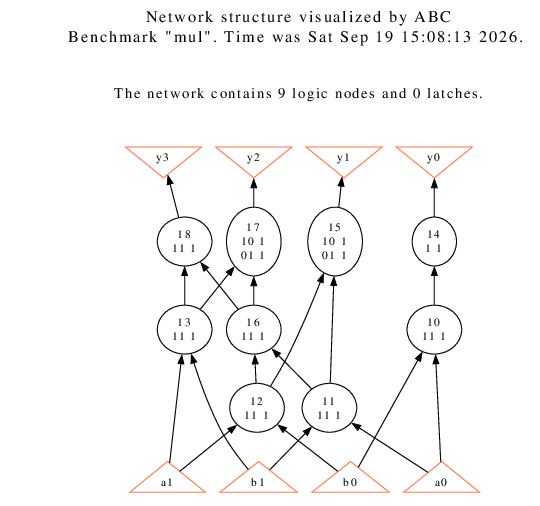
\includegraphics[width=0.72\textwidth]{report_figs/ex2_show_logic.png}
\caption{Network after \texttt{read} (\texttt{show}).}
\end{figure}

\begin{figure}[ht]
\centering
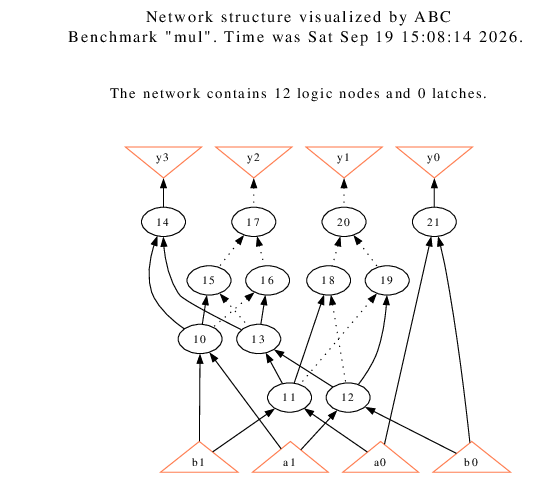
\includegraphics[width=0.72\textwidth]{report_figs/ex2_show_aig.png}
\caption{Structurally hashed AIG after \texttt{strash} (\texttt{show}).}
\end{figure}

\begin{figure}[ht]
\centering
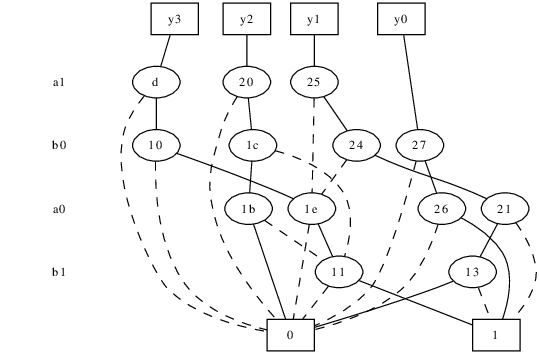
\includegraphics[width=0.72\textwidth]{report_figs/ex2_show_bdd.png}
\caption{Collapsed global BDDs after \texttt{collapse} (\texttt{show\_bdd -g}).}
\end{figure}

\section{Exercise 3: ABC Boolean Representations}

\subsection{3(a) Comparisons}

\paragraph{Logic network in AIG (\texttt{aig}) vs.\ structurally hashed AIG (\texttt{strash}).}
\mbox{}
\begin{lstlisting}
# after aig:
mul : i/o = 4/4  nd = 9  edge = 17  aig = 12  lev = 3
# after strash:
mul : i/o = 4/4  and = 12  lev = 4
\end{lstlisting}
Findings: \texttt{aig} keeps the original multi-level network topology and
stores each node's local function as a (possibly multi-gate) AIG fragment
(\texttt{nd=9}, \texttt{aig=12}). \texttt{strash} flattens everything into one
globally hashed AND-inverter graph (\texttt{and=12}). Structural hashing
merges identical gates, so the representation is unique and level count can
change.

\begin{figure}[ht]
\centering
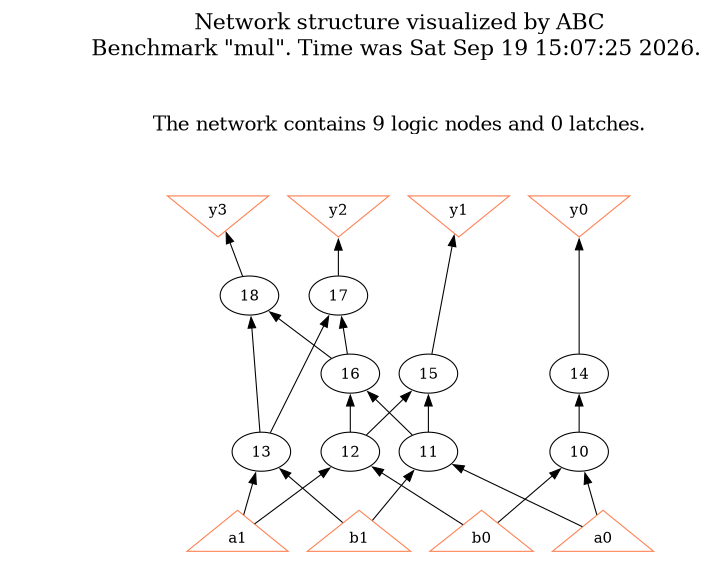
\includegraphics[width=0.45\textwidth]{report_figs/ex3_aig.png}
\hfill
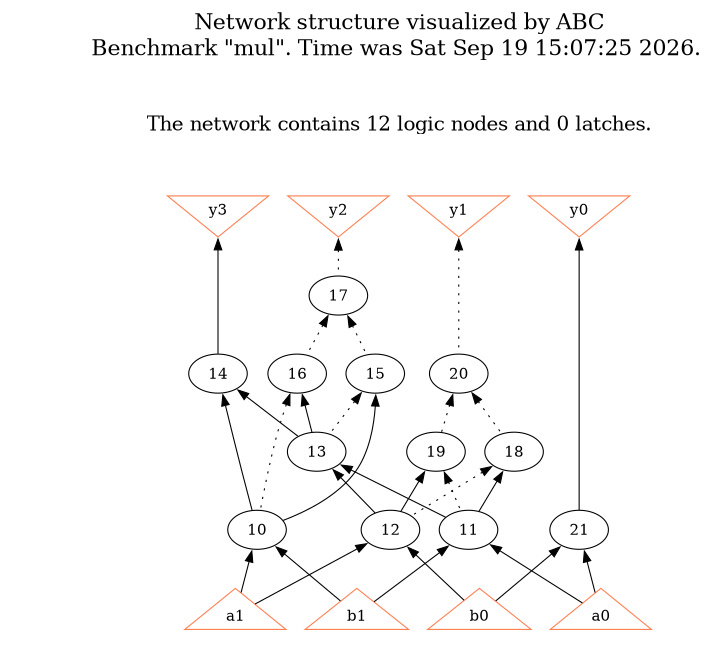
\includegraphics[width=0.45\textwidth]{report_figs/ex3_strash.png}
\caption{Left: after \texttt{aig}. Right: after \texttt{strash}.}
\end{figure}

\paragraph{Logic network in BDD (\texttt{bdd}) vs.\ collapsed BDD (\texttt{collapse}).}
\mbox{}
\begin{lstlisting}
# after bdd:
mul : i/o = 4/4  nd = 9  edge = 17  bdd = 16  lev = 3
# after collapse:
mul : i/o = 4/4  nd = 4  edge = 14  bdd = 14  lev = 1
\end{lstlisting}
Findings: \texttt{bdd} builds a local BDD for each internal node while
preserving the multi-level structure (\texttt{nd=9}, \texttt{lev=3}).
\texttt{collapse} builds global BDDs for the primary outputs only, eliminating
internal nodes (\texttt{nd=4} = four POs, \texttt{lev=1}).

\begin{figure}[ht]
\centering
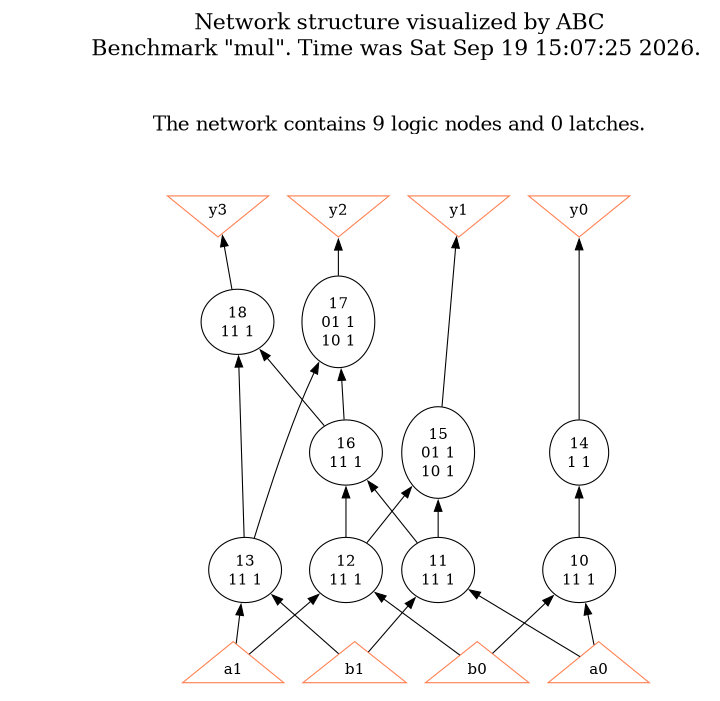
\includegraphics[width=0.45\textwidth]{report_figs/ex3_bdd.png}
\hfill
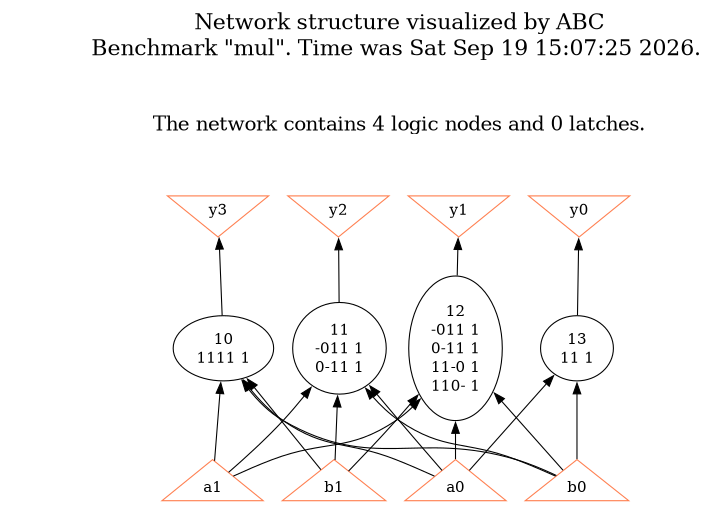
\includegraphics[width=0.45\textwidth]{report_figs/ex3_collapse.png}
\caption{Left: after \texttt{bdd}. Right: after \texttt{collapse}.}
\end{figure}

\FloatBarrier
\subsection{3(b) Strashed AIG $\rightarrow$ SOP logic network}

Command sequence:

\noindent\begin{minipage}{\linewidth}
\begin{lstlisting}
read lsv/pa1/mul.blif
strash
logic
sop
print_stats
\end{lstlisting}
\end{minipage}
Result:
\begin{lstlisting}
mul : i/o = 4/4  nd = 12  edge = 24  cube = 12  lev = 4
\end{lstlisting}
\texttt{logic} converts the structural AIG into a logic network;
\texttt{sop} expresses every node function in sum-of-products form
(\texttt{cube} appears in \texttt{print\_stats}). Verified with
\texttt{lsv\_print\_nodes}, which prints each node's SOP cubes.

\section{Exercise 4: Programming ABC (summary)}

Commands implemented under \texttt{src/ext-lsv/}:
\begin{itemize}
  \item \texttt{lsv\_cut\_tt <k>} --- irredundant $k$-feasible cuts + truth tables
  \item \texttt{lsv\_cut\_bddsize <k>} --- irredundant $k$-feasible cuts + ROBDD sizes
\end{itemize}

Verified against the handout Fig.~1 example (\texttt{lsv/pa1/example.blif}, $k=3$);
outputs match exactly. Dominated cuts are omitted (TA clarification on issue \#983).

\end{document}
